\subsection{Vectorization} \label{sec:vectorization}

%The vectorization stage transforms the pre-processed text of each error message into numeric information that quantitative techniques can digest.
%In particular, we leverage the \textbf{word2vec} language model \cite{mikolov2013word2vec} to compute token embeddings.
In the vectorization stage we leverage the \textbf{word2vec} language model \cite{mikolov2013word2vec} to compute message embeddings starting from pre-processed tokens.
Although more recent and powerful alternatives as the ones described in \cref{sec:related_opint} are available, they do not work well with short-text data \cite{albalawi2020short-text}. Thus, the simpler yet effective word2vec model is used here.

The idea behind word2vec is to find a convenient mapping between tokens (words) and a vectorial space where token linguistic relations are preserved, thus producing a distributed representation of words.
In this way, we obtain a numerical representation of textual data that quantitative algorithms can further process.
In particular, two alternative implementations of the word2vec model are available (see \cref{fig:word2vec}).
Both alternatives are based on a shallow (2-layer) neural network architecture and use a sliding window (context) of fixed size, $w$, around the current word, $w_t$.
The continuous bag-of-words (CBOW) model sets the learning objective to predict the current word from the surrounding context.
Conversely, the \mbox{skip-gram} model tries to guess the terms present in the context window starting from the current word.
To achieve that, the input words are first represented as 1-hot vectors of size $V$, where $V$ is the number of terms present in the corpus (vocabulary size). 
During this encoding step, a minimum allowed token frequency, $min\_count$ is set to discard terms appearing less than such threshold. This trick limits the vocabulary size by excluding rare tokens, thus lowering the computational requirements.
These input vectors pass through the first layer that projects them to a hidden space of customizable dimension, $h$. This mapping (embedding) is learned during the training phase such that terms often used together or in similar contexts should be projected nearby.
Finally, the resulting representations are put through the next network layer to get the predicted context (in the case of CBOW) or current words (skip-gram).

This work adopts the word2vec version exploiting the skip-gram architecture and uses its \texttt{pyspark} implementation.
Specifically, the model is trained on one month of data from 2020-10-01 to 2020-10-31.
In total, nearly 28.6 M error messages are analyzed, corresponding to a vocabulary of 970 unique tokens.
Once the model is trained, the resulting word embeddings are used to transform single tokens into numerical vectors, and they are then averaged to get the corresponding message representations.
Regarding hyper-parameters, the window size, the embedding size and the minimum count were the ones affecting the final representation the most.
For this reason, a grid-search is conducted to compare alternative parametrizations.  
The optimal configuration is then chosen based on the compactness of the resulting groups in the following clustering stage.
Specifically, the values of $w=12$, $h=300$ and $min\_count=50$ seem to work best in our use case.

\begin{figure}
    \centering
    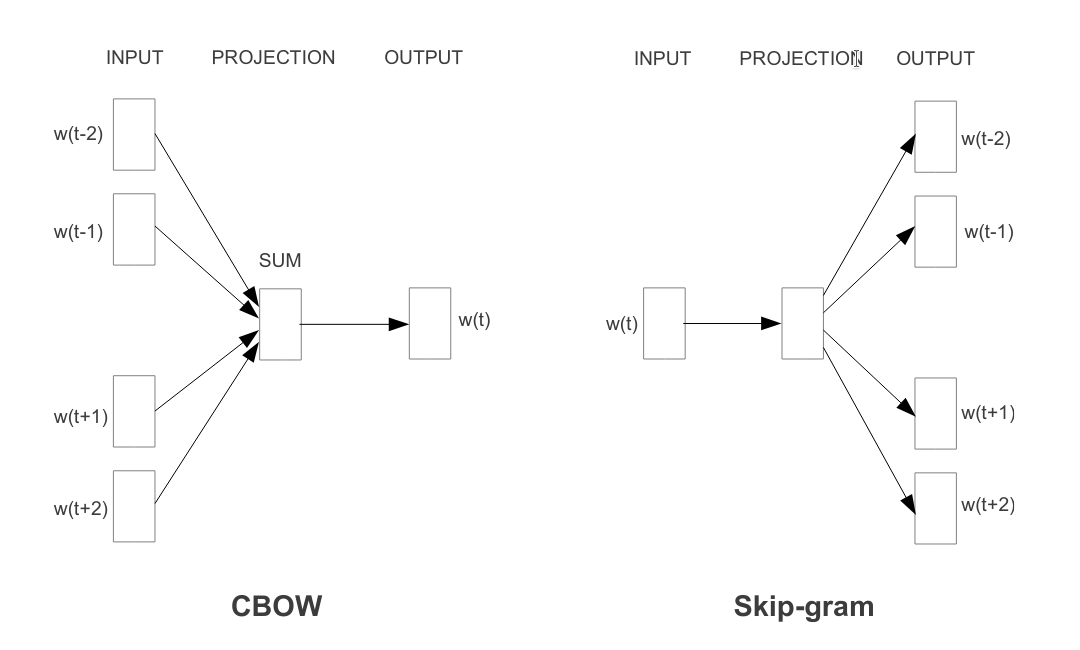
\includegraphics[width=\textwidth]{figures/410_method/word2vec.png}
    \caption{\textbf{Word2vec model architectures.} The CBOW architecture predicts the current word based on the
context, and the Skip-gram predicts surrounding words given the current word. The figure is borrowed from the original paper \protect \cite{mikolov2013word2vec}
}
    \label{fig:word2vec}
\end{figure}